
%(BEGIN_QUESTION)
% Copyright 2015, Tony R. Kuphaldt, released under the Creative Commons Attribution License (v 1.0)
% This means you may do almost anything with this work of mine, so long as you give me proper credit

A technician needs to write a program for an Allen-Bradley CompactLogix PLC to control a pressure-relieving solenoid valve in a gas processing system.  A pair of high-pressure control switches signals the PLC when to open the solenoid valve: one telling the PLC to open the valve after a 3-second time delay and the other (called the ``high-high'' switch, with a higher trip setting) telling the PLC to open the valve immediately.  A pushbutton switch serves as a manual override to open the solenoid valve immediately when pressed.  In all cases, the solenoid vent valve will remain open (energized) until pressure falls below the setting of a low-pressure gas switch.  The operating statuses of these switches are listed here:

\begin{itemize}
\item{} {\bf Override pushbutton} (normally-open): open when unpressed, closed when pressed
\item{} {\bf Low gas pressure} (normally-closed): closed when pressure is less than 10 PSI, open when pressure exceeds 10 PSI
\item{} {\bf High gas pressure} (normally-closed): closed when pressure is less than 30 PSI, open when pressure exceeds 30 PSI
\item{} {\bf High-high gas pressure} (normally-open): open when pressure is less than 40 PSI, closed when pressure exceeds 40 PSI
\end{itemize}

The technician's first attempt is shown here, but it contains a serious error.  Identify and correct this error:

$$\includegraphics[width=15.5cm]{i02853x01.eps}$$

\underbar{file i02853}
%(END_QUESTION)





%(BEGIN_ANSWER)

The {\tt High\_pressure} contact instruction should be drawn as normally-closed rather than normally-open as shown in the technician's first draft of the PLC program.  This particular switch signals a high-pressure condition by opening its contacts, since the real-world switch is normally-closed (NC).  We want the 3-second timer to begin timing when this switch senses a high pressure, and so we need the contact instruction to color when the real-world high-pressure switch trips (opens).  A PLC contact instruction that colors when it senses a ``0'' bit condition is a normally-closed (NC) instruction.

%(END_ANSWER)





%(BEGIN_NOTES)


%INDEX% PLC, diagnosing programming error
%INDEX% PLC, relating I/O status to virtual elements (troubleshooting)
%INDEX% PLC, troubleshooting: motor start/stop control circuit

%(END_NOTES)


